
% Default to the notebook output style

    


% Inherit from the specified cell style.




    
\documentclass[11pt]{article}

    
    
    \usepackage[T1]{fontenc}
    % Nicer default font (+ math font) than Computer Modern for most use cases
    \usepackage{mathpazo}

    % Basic figure setup, for now with no caption control since it's done
    % automatically by Pandoc (which extracts ![](path) syntax from Markdown).
    \usepackage{graphicx}
    % We will generate all images so they have a width \maxwidth. This means
    % that they will get their normal width if they fit onto the page, but
    % are scaled down if they would overflow the margins.
    \makeatletter
    \def\maxwidth{\ifdim\Gin@nat@width>\linewidth\linewidth
    \else\Gin@nat@width\fi}
    \makeatother
    \let\Oldincludegraphics\includegraphics
    % Set max figure width to be 80% of text width, for now hardcoded.
    \renewcommand{\includegraphics}[1]{\Oldincludegraphics[width=.8\maxwidth]{#1}}
    % Ensure that by default, figures have no caption (until we provide a
    % proper Figure object with a Caption API and a way to capture that
    % in the conversion process - todo).
    \usepackage{caption}
    \DeclareCaptionLabelFormat{nolabel}{}
    \captionsetup{labelformat=nolabel}

    \usepackage{adjustbox} % Used to constrain images to a maximum size 
    \usepackage{xcolor} % Allow colors to be defined
    \usepackage{enumerate} % Needed for markdown enumerations to work
    \usepackage{geometry} % Used to adjust the document margins
    \usepackage{amsmath} % Equations
    \usepackage{amssymb} % Equations
    \usepackage{textcomp} % defines textquotesingle
    % Hack from http://tex.stackexchange.com/a/47451/13684:
    \AtBeginDocument{%
        \def\PYZsq{\textquotesingle}% Upright quotes in Pygmentized code
    }
    \usepackage{upquote} % Upright quotes for verbatim code
    \usepackage{eurosym} % defines \euro
    \usepackage[mathletters]{ucs} % Extended unicode (utf-8) support
    \usepackage[utf8x]{inputenc} % Allow utf-8 characters in the tex document
    \usepackage{fancyvrb} % verbatim replacement that allows latex
    \usepackage{grffile} % extends the file name processing of package graphics 
                         % to support a larger range 
    % The hyperref package gives us a pdf with properly built
    % internal navigation ('pdf bookmarks' for the table of contents,
    % internal cross-reference links, web links for URLs, etc.)
    \usepackage{hyperref}
    \usepackage{longtable} % longtable support required by pandoc >1.10
    \usepackage{booktabs}  % table support for pandoc > 1.12.2
    \usepackage[inline]{enumitem} % IRkernel/repr support (it uses the enumerate* environment)
    \usepackage[normalem]{ulem} % ulem is needed to support strikethroughs (\sout)
                                % normalem makes italics be italics, not underlines
    

    
    
    % Colors for the hyperref package
    \definecolor{urlcolor}{rgb}{0,.145,.698}
    \definecolor{linkcolor}{rgb}{.71,0.21,0.01}
    \definecolor{citecolor}{rgb}{.12,.54,.11}

    % ANSI colors
    \definecolor{ansi-black}{HTML}{3E424D}
    \definecolor{ansi-black-intense}{HTML}{282C36}
    \definecolor{ansi-red}{HTML}{E75C58}
    \definecolor{ansi-red-intense}{HTML}{B22B31}
    \definecolor{ansi-green}{HTML}{00A250}
    \definecolor{ansi-green-intense}{HTML}{007427}
    \definecolor{ansi-yellow}{HTML}{DDB62B}
    \definecolor{ansi-yellow-intense}{HTML}{B27D12}
    \definecolor{ansi-blue}{HTML}{208FFB}
    \definecolor{ansi-blue-intense}{HTML}{0065CA}
    \definecolor{ansi-magenta}{HTML}{D160C4}
    \definecolor{ansi-magenta-intense}{HTML}{A03196}
    \definecolor{ansi-cyan}{HTML}{60C6C8}
    \definecolor{ansi-cyan-intense}{HTML}{258F8F}
    \definecolor{ansi-white}{HTML}{C5C1B4}
    \definecolor{ansi-white-intense}{HTML}{A1A6B2}

    % commands and environments needed by pandoc snippets
    % extracted from the output of `pandoc -s`
    \providecommand{\tightlist}{%
      \setlength{\itemsep}{0pt}\setlength{\parskip}{0pt}}
    \DefineVerbatimEnvironment{Highlighting}{Verbatim}{commandchars=\\\{\}}
    % Add ',fontsize=\small' for more characters per line
    \newenvironment{Shaded}{}{}
    \newcommand{\KeywordTok}[1]{\textcolor[rgb]{0.00,0.44,0.13}{\textbf{{#1}}}}
    \newcommand{\DataTypeTok}[1]{\textcolor[rgb]{0.56,0.13,0.00}{{#1}}}
    \newcommand{\DecValTok}[1]{\textcolor[rgb]{0.25,0.63,0.44}{{#1}}}
    \newcommand{\BaseNTok}[1]{\textcolor[rgb]{0.25,0.63,0.44}{{#1}}}
    \newcommand{\FloatTok}[1]{\textcolor[rgb]{0.25,0.63,0.44}{{#1}}}
    \newcommand{\CharTok}[1]{\textcolor[rgb]{0.25,0.44,0.63}{{#1}}}
    \newcommand{\StringTok}[1]{\textcolor[rgb]{0.25,0.44,0.63}{{#1}}}
    \newcommand{\CommentTok}[1]{\textcolor[rgb]{0.38,0.63,0.69}{\textit{{#1}}}}
    \newcommand{\OtherTok}[1]{\textcolor[rgb]{0.00,0.44,0.13}{{#1}}}
    \newcommand{\AlertTok}[1]{\textcolor[rgb]{1.00,0.00,0.00}{\textbf{{#1}}}}
    \newcommand{\FunctionTok}[1]{\textcolor[rgb]{0.02,0.16,0.49}{{#1}}}
    \newcommand{\RegionMarkerTok}[1]{{#1}}
    \newcommand{\ErrorTok}[1]{\textcolor[rgb]{1.00,0.00,0.00}{\textbf{{#1}}}}
    \newcommand{\NormalTok}[1]{{#1}}
    
    % Additional commands for more recent versions of Pandoc
    \newcommand{\ConstantTok}[1]{\textcolor[rgb]{0.53,0.00,0.00}{{#1}}}
    \newcommand{\SpecialCharTok}[1]{\textcolor[rgb]{0.25,0.44,0.63}{{#1}}}
    \newcommand{\VerbatimStringTok}[1]{\textcolor[rgb]{0.25,0.44,0.63}{{#1}}}
    \newcommand{\SpecialStringTok}[1]{\textcolor[rgb]{0.73,0.40,0.53}{{#1}}}
    \newcommand{\ImportTok}[1]{{#1}}
    \newcommand{\DocumentationTok}[1]{\textcolor[rgb]{0.73,0.13,0.13}{\textit{{#1}}}}
    \newcommand{\AnnotationTok}[1]{\textcolor[rgb]{0.38,0.63,0.69}{\textbf{\textit{{#1}}}}}
    \newcommand{\CommentVarTok}[1]{\textcolor[rgb]{0.38,0.63,0.69}{\textbf{\textit{{#1}}}}}
    \newcommand{\VariableTok}[1]{\textcolor[rgb]{0.10,0.09,0.49}{{#1}}}
    \newcommand{\ControlFlowTok}[1]{\textcolor[rgb]{0.00,0.44,0.13}{\textbf{{#1}}}}
    \newcommand{\OperatorTok}[1]{\textcolor[rgb]{0.40,0.40,0.40}{{#1}}}
    \newcommand{\BuiltInTok}[1]{{#1}}
    \newcommand{\ExtensionTok}[1]{{#1}}
    \newcommand{\PreprocessorTok}[1]{\textcolor[rgb]{0.74,0.48,0.00}{{#1}}}
    \newcommand{\AttributeTok}[1]{\textcolor[rgb]{0.49,0.56,0.16}{{#1}}}
    \newcommand{\InformationTok}[1]{\textcolor[rgb]{0.38,0.63,0.69}{\textbf{\textit{{#1}}}}}
    \newcommand{\WarningTok}[1]{\textcolor[rgb]{0.38,0.63,0.69}{\textbf{\textit{{#1}}}}}
    
    
    % Define a nice break command that doesn't care if a line doesn't already
    % exist.
    \def\br{\hspace*{\fill} \\* }
    % Math Jax compatability definitions
    \def\gt{>}
    \def\lt{<}
    % Document parameters
    \title{07\_reverberation}
    
    
    

    % Pygments definitions
    
\makeatletter
\def\PY@reset{\let\PY@it=\relax \let\PY@bf=\relax%
    \let\PY@ul=\relax \let\PY@tc=\relax%
    \let\PY@bc=\relax \let\PY@ff=\relax}
\def\PY@tok#1{\csname PY@tok@#1\endcsname}
\def\PY@toks#1+{\ifx\relax#1\empty\else%
    \PY@tok{#1}\expandafter\PY@toks\fi}
\def\PY@do#1{\PY@bc{\PY@tc{\PY@ul{%
    \PY@it{\PY@bf{\PY@ff{#1}}}}}}}
\def\PY#1#2{\PY@reset\PY@toks#1+\relax+\PY@do{#2}}

\expandafter\def\csname PY@tok@w\endcsname{\def\PY@tc##1{\textcolor[rgb]{0.73,0.73,0.73}{##1}}}
\expandafter\def\csname PY@tok@c\endcsname{\let\PY@it=\textit\def\PY@tc##1{\textcolor[rgb]{0.25,0.50,0.50}{##1}}}
\expandafter\def\csname PY@tok@cp\endcsname{\def\PY@tc##1{\textcolor[rgb]{0.74,0.48,0.00}{##1}}}
\expandafter\def\csname PY@tok@k\endcsname{\let\PY@bf=\textbf\def\PY@tc##1{\textcolor[rgb]{0.00,0.50,0.00}{##1}}}
\expandafter\def\csname PY@tok@kp\endcsname{\def\PY@tc##1{\textcolor[rgb]{0.00,0.50,0.00}{##1}}}
\expandafter\def\csname PY@tok@kt\endcsname{\def\PY@tc##1{\textcolor[rgb]{0.69,0.00,0.25}{##1}}}
\expandafter\def\csname PY@tok@o\endcsname{\def\PY@tc##1{\textcolor[rgb]{0.40,0.40,0.40}{##1}}}
\expandafter\def\csname PY@tok@ow\endcsname{\let\PY@bf=\textbf\def\PY@tc##1{\textcolor[rgb]{0.67,0.13,1.00}{##1}}}
\expandafter\def\csname PY@tok@nb\endcsname{\def\PY@tc##1{\textcolor[rgb]{0.00,0.50,0.00}{##1}}}
\expandafter\def\csname PY@tok@nf\endcsname{\def\PY@tc##1{\textcolor[rgb]{0.00,0.00,1.00}{##1}}}
\expandafter\def\csname PY@tok@nc\endcsname{\let\PY@bf=\textbf\def\PY@tc##1{\textcolor[rgb]{0.00,0.00,1.00}{##1}}}
\expandafter\def\csname PY@tok@nn\endcsname{\let\PY@bf=\textbf\def\PY@tc##1{\textcolor[rgb]{0.00,0.00,1.00}{##1}}}
\expandafter\def\csname PY@tok@ne\endcsname{\let\PY@bf=\textbf\def\PY@tc##1{\textcolor[rgb]{0.82,0.25,0.23}{##1}}}
\expandafter\def\csname PY@tok@nv\endcsname{\def\PY@tc##1{\textcolor[rgb]{0.10,0.09,0.49}{##1}}}
\expandafter\def\csname PY@tok@no\endcsname{\def\PY@tc##1{\textcolor[rgb]{0.53,0.00,0.00}{##1}}}
\expandafter\def\csname PY@tok@nl\endcsname{\def\PY@tc##1{\textcolor[rgb]{0.63,0.63,0.00}{##1}}}
\expandafter\def\csname PY@tok@ni\endcsname{\let\PY@bf=\textbf\def\PY@tc##1{\textcolor[rgb]{0.60,0.60,0.60}{##1}}}
\expandafter\def\csname PY@tok@na\endcsname{\def\PY@tc##1{\textcolor[rgb]{0.49,0.56,0.16}{##1}}}
\expandafter\def\csname PY@tok@nt\endcsname{\let\PY@bf=\textbf\def\PY@tc##1{\textcolor[rgb]{0.00,0.50,0.00}{##1}}}
\expandafter\def\csname PY@tok@nd\endcsname{\def\PY@tc##1{\textcolor[rgb]{0.67,0.13,1.00}{##1}}}
\expandafter\def\csname PY@tok@s\endcsname{\def\PY@tc##1{\textcolor[rgb]{0.73,0.13,0.13}{##1}}}
\expandafter\def\csname PY@tok@sd\endcsname{\let\PY@it=\textit\def\PY@tc##1{\textcolor[rgb]{0.73,0.13,0.13}{##1}}}
\expandafter\def\csname PY@tok@si\endcsname{\let\PY@bf=\textbf\def\PY@tc##1{\textcolor[rgb]{0.73,0.40,0.53}{##1}}}
\expandafter\def\csname PY@tok@se\endcsname{\let\PY@bf=\textbf\def\PY@tc##1{\textcolor[rgb]{0.73,0.40,0.13}{##1}}}
\expandafter\def\csname PY@tok@sr\endcsname{\def\PY@tc##1{\textcolor[rgb]{0.73,0.40,0.53}{##1}}}
\expandafter\def\csname PY@tok@ss\endcsname{\def\PY@tc##1{\textcolor[rgb]{0.10,0.09,0.49}{##1}}}
\expandafter\def\csname PY@tok@sx\endcsname{\def\PY@tc##1{\textcolor[rgb]{0.00,0.50,0.00}{##1}}}
\expandafter\def\csname PY@tok@m\endcsname{\def\PY@tc##1{\textcolor[rgb]{0.40,0.40,0.40}{##1}}}
\expandafter\def\csname PY@tok@gh\endcsname{\let\PY@bf=\textbf\def\PY@tc##1{\textcolor[rgb]{0.00,0.00,0.50}{##1}}}
\expandafter\def\csname PY@tok@gu\endcsname{\let\PY@bf=\textbf\def\PY@tc##1{\textcolor[rgb]{0.50,0.00,0.50}{##1}}}
\expandafter\def\csname PY@tok@gd\endcsname{\def\PY@tc##1{\textcolor[rgb]{0.63,0.00,0.00}{##1}}}
\expandafter\def\csname PY@tok@gi\endcsname{\def\PY@tc##1{\textcolor[rgb]{0.00,0.63,0.00}{##1}}}
\expandafter\def\csname PY@tok@gr\endcsname{\def\PY@tc##1{\textcolor[rgb]{1.00,0.00,0.00}{##1}}}
\expandafter\def\csname PY@tok@ge\endcsname{\let\PY@it=\textit}
\expandafter\def\csname PY@tok@gs\endcsname{\let\PY@bf=\textbf}
\expandafter\def\csname PY@tok@gp\endcsname{\let\PY@bf=\textbf\def\PY@tc##1{\textcolor[rgb]{0.00,0.00,0.50}{##1}}}
\expandafter\def\csname PY@tok@go\endcsname{\def\PY@tc##1{\textcolor[rgb]{0.53,0.53,0.53}{##1}}}
\expandafter\def\csname PY@tok@gt\endcsname{\def\PY@tc##1{\textcolor[rgb]{0.00,0.27,0.87}{##1}}}
\expandafter\def\csname PY@tok@err\endcsname{\def\PY@bc##1{\setlength{\fboxsep}{0pt}\fcolorbox[rgb]{1.00,0.00,0.00}{1,1,1}{\strut ##1}}}
\expandafter\def\csname PY@tok@kc\endcsname{\let\PY@bf=\textbf\def\PY@tc##1{\textcolor[rgb]{0.00,0.50,0.00}{##1}}}
\expandafter\def\csname PY@tok@kd\endcsname{\let\PY@bf=\textbf\def\PY@tc##1{\textcolor[rgb]{0.00,0.50,0.00}{##1}}}
\expandafter\def\csname PY@tok@kn\endcsname{\let\PY@bf=\textbf\def\PY@tc##1{\textcolor[rgb]{0.00,0.50,0.00}{##1}}}
\expandafter\def\csname PY@tok@kr\endcsname{\let\PY@bf=\textbf\def\PY@tc##1{\textcolor[rgb]{0.00,0.50,0.00}{##1}}}
\expandafter\def\csname PY@tok@bp\endcsname{\def\PY@tc##1{\textcolor[rgb]{0.00,0.50,0.00}{##1}}}
\expandafter\def\csname PY@tok@fm\endcsname{\def\PY@tc##1{\textcolor[rgb]{0.00,0.00,1.00}{##1}}}
\expandafter\def\csname PY@tok@vc\endcsname{\def\PY@tc##1{\textcolor[rgb]{0.10,0.09,0.49}{##1}}}
\expandafter\def\csname PY@tok@vg\endcsname{\def\PY@tc##1{\textcolor[rgb]{0.10,0.09,0.49}{##1}}}
\expandafter\def\csname PY@tok@vi\endcsname{\def\PY@tc##1{\textcolor[rgb]{0.10,0.09,0.49}{##1}}}
\expandafter\def\csname PY@tok@vm\endcsname{\def\PY@tc##1{\textcolor[rgb]{0.10,0.09,0.49}{##1}}}
\expandafter\def\csname PY@tok@sa\endcsname{\def\PY@tc##1{\textcolor[rgb]{0.73,0.13,0.13}{##1}}}
\expandafter\def\csname PY@tok@sb\endcsname{\def\PY@tc##1{\textcolor[rgb]{0.73,0.13,0.13}{##1}}}
\expandafter\def\csname PY@tok@sc\endcsname{\def\PY@tc##1{\textcolor[rgb]{0.73,0.13,0.13}{##1}}}
\expandafter\def\csname PY@tok@dl\endcsname{\def\PY@tc##1{\textcolor[rgb]{0.73,0.13,0.13}{##1}}}
\expandafter\def\csname PY@tok@s2\endcsname{\def\PY@tc##1{\textcolor[rgb]{0.73,0.13,0.13}{##1}}}
\expandafter\def\csname PY@tok@sh\endcsname{\def\PY@tc##1{\textcolor[rgb]{0.73,0.13,0.13}{##1}}}
\expandafter\def\csname PY@tok@s1\endcsname{\def\PY@tc##1{\textcolor[rgb]{0.73,0.13,0.13}{##1}}}
\expandafter\def\csname PY@tok@mb\endcsname{\def\PY@tc##1{\textcolor[rgb]{0.40,0.40,0.40}{##1}}}
\expandafter\def\csname PY@tok@mf\endcsname{\def\PY@tc##1{\textcolor[rgb]{0.40,0.40,0.40}{##1}}}
\expandafter\def\csname PY@tok@mh\endcsname{\def\PY@tc##1{\textcolor[rgb]{0.40,0.40,0.40}{##1}}}
\expandafter\def\csname PY@tok@mi\endcsname{\def\PY@tc##1{\textcolor[rgb]{0.40,0.40,0.40}{##1}}}
\expandafter\def\csname PY@tok@il\endcsname{\def\PY@tc##1{\textcolor[rgb]{0.40,0.40,0.40}{##1}}}
\expandafter\def\csname PY@tok@mo\endcsname{\def\PY@tc##1{\textcolor[rgb]{0.40,0.40,0.40}{##1}}}
\expandafter\def\csname PY@tok@ch\endcsname{\let\PY@it=\textit\def\PY@tc##1{\textcolor[rgb]{0.25,0.50,0.50}{##1}}}
\expandafter\def\csname PY@tok@cm\endcsname{\let\PY@it=\textit\def\PY@tc##1{\textcolor[rgb]{0.25,0.50,0.50}{##1}}}
\expandafter\def\csname PY@tok@cpf\endcsname{\let\PY@it=\textit\def\PY@tc##1{\textcolor[rgb]{0.25,0.50,0.50}{##1}}}
\expandafter\def\csname PY@tok@c1\endcsname{\let\PY@it=\textit\def\PY@tc##1{\textcolor[rgb]{0.25,0.50,0.50}{##1}}}
\expandafter\def\csname PY@tok@cs\endcsname{\let\PY@it=\textit\def\PY@tc##1{\textcolor[rgb]{0.25,0.50,0.50}{##1}}}

\def\PYZbs{\char`\\}
\def\PYZus{\char`\_}
\def\PYZob{\char`\{}
\def\PYZcb{\char`\}}
\def\PYZca{\char`\^}
\def\PYZam{\char`\&}
\def\PYZlt{\char`\<}
\def\PYZgt{\char`\>}
\def\PYZsh{\char`\#}
\def\PYZpc{\char`\%}
\def\PYZdl{\char`\$}
\def\PYZhy{\char`\-}
\def\PYZsq{\char`\'}
\def\PYZdq{\char`\"}
\def\PYZti{\char`\~}
% for compatibility with earlier versions
\def\PYZat{@}
\def\PYZlb{[}
\def\PYZrb{]}
\makeatother


    % Exact colors from NB
    \definecolor{incolor}{rgb}{0.0, 0.0, 0.5}
    \definecolor{outcolor}{rgb}{0.545, 0.0, 0.0}



    
    % Prevent overflowing lines due to hard-to-break entities
    \sloppy 
    % Setup hyperref package
    \hypersetup{
      breaklinks=true,  % so long urls are correctly broken across lines
      colorlinks=true,
      urlcolor=urlcolor,
      linkcolor=linkcolor,
      citecolor=citecolor,
      }
    % Slightly bigger margins than the latex defaults
    
    \geometry{verbose,tmargin=1in,bmargin=1in,lmargin=1in,rmargin=1in}
    
    

    \begin{document}
    
    
    \maketitle
    
    

    
    \hypertarget{reverberation-and-3-d-sounds}{%
\section{Reverberation and 3-D
sounds}\label{reverberation-and-3-d-sounds}}

Sounds people are exposed in natural life have various kinds of
reverberation. Today as sounds are synthesized and recorded in an
anechoic environments, it is crucial to add reverberation to emulate
``true'' sounds. Film/game/VR/Music industry have been investing in
artificial reverberation to make better sound experience.

Reverberation is a consquence of the slowness in sound; sound travels in
the air at approximately 345 m/s.

\begin{figure}
\centering
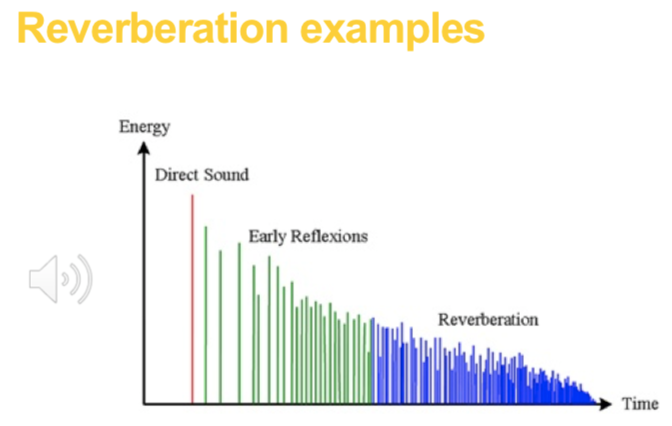
\includegraphics{images/reverb_example.png}
\caption{reverb\_example}
\end{figure}

    \hypertarget{techniques}{%
\subsection{Techniques}\label{techniques}}

\hypertarget{traditional-techniques}{%
\subsubsection{Traditional techniques}\label{traditional-techniques}}

Traditional techiniques involve physical space to generate
reverberation. As the reverberation is real, not simulated, the result
sound is rich and natural. It is not used in practice anymore due to its
inherent constraints: un-simulatable and unflexibility.

Types:

\begin{itemize}
\tightlist
\item
  Echo chambers
\item
  Electromechanical reverb

  \begin{itemize}
  \tightlist
  \item
    Plates
  \item
    Spring
  \end{itemize}
\end{itemize}

\hypertarget{analog-reverberation}{%
\subsubsection{Analog reverberation}\label{analog-reverberation}}

There are tape and oil reverbers used in the 20th century but are not
used anymore

\hypertarget{algorithmic-techniques}{%
\subsubsection{Algorithmic techniques}\label{algorithmic-techniques}}

\begin{itemize}
\tightlist
\item
  Comb filter (recirculating delay line)
\item
  Schroeder All-Pass filter

  \begin{itemize}
  \tightlist
  \item
    Add a negative feedforward path to flatten the spectrum of a comb
    filter
  \item
    Long impulse response, such as that of a comb filter
  \end{itemize}
\item
  Moorer reverb

  \begin{itemize}
  \tightlist
  \item
    Lowpass-comb filter
  \end{itemize}
\item
  Feedback Delay Netowrks (FDN)
\item
  Convolution Reverb
\item
  Modal reverb
\item
  Scattering Delay Network
\end{itemize}

    \hypertarget{places-with-unintended-reverberation}{%
\subsection{Places with unintended
reverberation}\label{places-with-unintended-reverberation}}

Kukulkan temple generates reverberation which is similar to flanging.
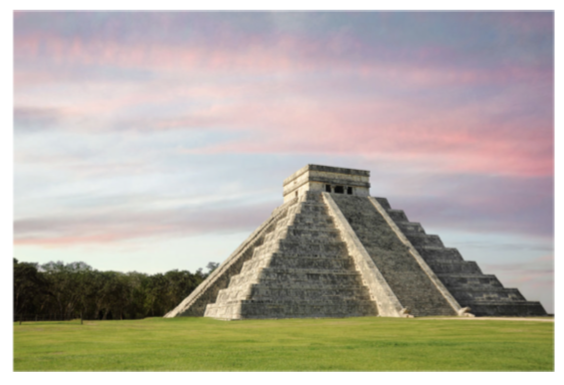
\includegraphics{images/kukulkan.png}
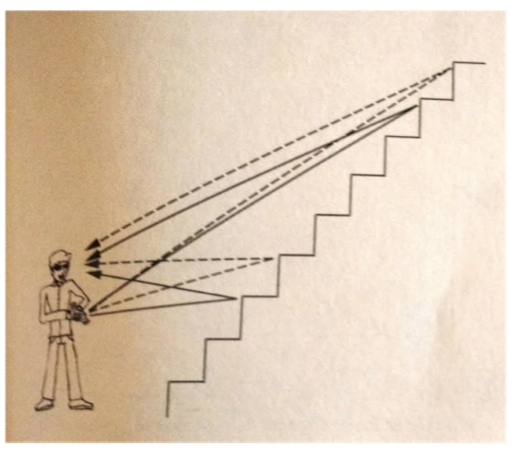
\includegraphics{images/kukulkan2.png}

This gallery propagates sound so that a person on the other side of the
wall hears you as if you were standing next her.
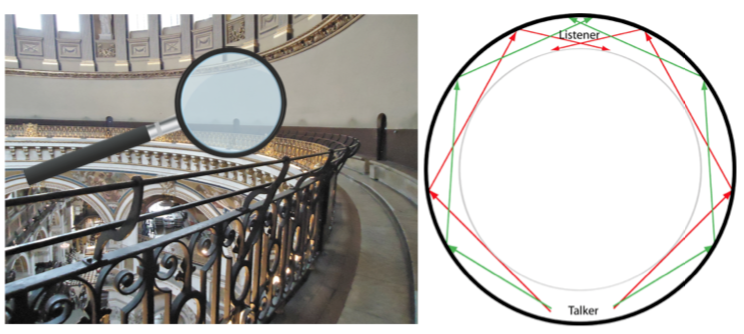
\includegraphics{images/whispering_gallery.png}

    \hypertarget{comb-reverberation-code}{%
\subsection{Comb Reverberation Code}\label{comb-reverberation-code}}

Here is a difference equation of an FIR comb filter:

\[y(n)=x(n)+g x(n-M)\]

where,

\[M=\tau / f_{S}\]

Here is the system function in Z domain:

\[H(z)=1+g z^{-M}\]

    \begin{Verbatim}[commandchars=\\\{\}]
{\color{incolor}In [{\color{incolor}32}]:} \PY{k+kn}{from} \PY{n+nn}{\PYZus{}\PYZus{}future\PYZus{}\PYZus{}} \PY{k}{import} \PY{n}{print\PYZus{}function}
         \PY{k+kn}{from} \PY{n+nn}{scipy}\PY{n+nn}{.}\PY{n+nn}{signal} \PY{k}{import} \PY{n}{freqz}\PY{p}{,} \PY{n}{lfilter}
         
         \PY{k+kn}{from} \PY{n+nn}{asp} \PY{k}{import} \PY{n}{config}
         \PY{k+kn}{import} \PY{n+nn}{numpy} \PY{k}{as} \PY{n+nn}{np}
         \PY{k+kn}{from} \PY{n+nn}{asp}\PY{n+nn}{.}\PY{n+nn}{core} \PY{k}{import} \PY{n}{read\PYZus{}wave}\PY{p}{,} \PY{n}{Wave}
         \PY{k+kn}{from} \PY{n+nn}{IPython}\PY{n+nn}{.}\PY{n+nn}{display} \PY{k}{import} \PY{n}{Audio}
\end{Verbatim}


    \begin{Verbatim}[commandchars=\\\{\}]
{\color{incolor}In [{\color{incolor}3}]:} \PY{n}{config}\PY{o}{.}\PY{n}{paths}\PY{o}{.}\PY{n}{data}
\end{Verbatim}


\begin{Verbatim}[commandchars=\\\{\}]
{\color{outcolor}Out[{\color{outcolor}3}]:} ['/Users/parks1/asp/data/c2e2f2.wav',
         '/Users/parks1/asp/data/c2e2.wav',
         '/Users/parks1/asp/data/92002\_\_jcveliz\_\_violin-origional.wav',
         '/Users/parks1/asp/data/c2e2g2.wav']
\end{Verbatim}
            
    Load audio sample

    \begin{Verbatim}[commandchars=\\\{\}]
{\color{incolor}In [{\color{incolor}73}]:} \PY{n}{violin} \PY{o}{=} \PY{n}{read\PYZus{}wave}\PY{p}{(}\PY{n}{config}\PY{o}{.}\PY{n}{paths}\PY{o}{.}\PY{n}{data}\PY{p}{[}\PY{l+m+mi}{2}\PY{p}{]}\PY{p}{)}
         \PY{n}{y\PYZus{}reference} \PY{o}{=} \PY{n}{violin}\PY{o}{.}\PY{n}{ys}
         \PY{n}{violin}\PY{o}{.}\PY{n}{make\PYZus{}audio}\PY{p}{(}\PY{p}{)}
\end{Verbatim}


\begin{Verbatim}[commandchars=\\\{\}]
{\color{outcolor}Out[{\color{outcolor}73}]:} <IPython.lib.display.Audio object>
\end{Verbatim}
            
    Comb filter in time domain

    \begin{Verbatim}[commandchars=\\\{\}]
{\color{incolor}In [{\color{incolor}18}]:} \PY{k}{def} \PY{n+nf}{comb\PYZus{}filter}\PY{p}{(}\PY{n}{ys}\PY{p}{,} \PY{n}{M}\PY{p}{,} \PY{n}{gain}\PY{o}{=}\PY{l+m+mf}{0.7}\PY{p}{)}\PY{p}{:}
             \PY{k}{return} \PY{n}{ys}\PY{p}{[}\PY{n}{M}\PY{p}{:}\PY{p}{]} \PY{o}{+} \PY{n}{gain} \PY{o}{*} \PY{n}{ys}\PY{p}{[}\PY{p}{:}\PY{o}{\PYZhy{}}\PY{n}{M}\PY{p}{]}
             
         \PY{n}{violin}\PY{o}{.}\PY{n}{ys} \PY{o}{=} \PY{n}{comb\PYZus{}filter}\PY{p}{(}\PY{n}{violin}\PY{o}{.}\PY{n}{ys}\PY{p}{,} \PY{l+m+mi}{4410}\PY{p}{)}
         \PY{n}{violin}\PY{o}{.}\PY{n}{make\PYZus{}audio}\PY{p}{(}\PY{p}{)}
\end{Verbatim}


\begin{Verbatim}[commandchars=\\\{\}]
{\color{outcolor}Out[{\color{outcolor}18}]:} <IPython.lib.display.Audio object>
\end{Verbatim}
            
    Comb filter in Z domain

    \begin{Verbatim}[commandchars=\\\{\}]
{\color{incolor}In [{\color{incolor}31}]:} \PY{k}{def} \PY{n+nf}{comb\PYZus{}filter\PYZus{}z}\PY{p}{(}\PY{n}{ys}\PY{p}{,} \PY{n}{M}\PY{p}{,} \PY{n}{gain}\PY{o}{=}\PY{l+m+mf}{0.7}\PY{p}{)}\PY{p}{:}
             \PY{c+c1}{\PYZsh{} B is the feedforward part}
             \PY{n}{b} \PY{o}{=} \PY{n}{np}\PY{o}{.}\PY{n}{zeros}\PY{p}{(}\PY{n}{M}\PY{o}{+}\PY{l+m+mi}{1}\PY{p}{)}
             \PY{n}{b}\PY{p}{[}\PY{n}{M}\PY{p}{]} \PY{o}{=} \PY{n}{gain}
             \PY{n}{b}\PY{p}{[}\PY{l+m+mi}{0}\PY{p}{]} \PY{o}{=} \PY{l+m+mi}{1}
             
             \PY{k}{return} \PY{n}{lfilter}\PY{p}{(}\PY{n}{b}\PY{p}{,} \PY{p}{[}\PY{l+m+mi}{1}\PY{p}{]}\PY{p}{,} \PY{n}{ys}\PY{p}{)}
             
         \PY{n}{violin}\PY{o}{.}\PY{n}{ys} \PY{o}{=} \PY{n}{comb\PYZus{}filter\PYZus{}z}\PY{p}{(}\PY{n}{violin}\PY{o}{.}\PY{n}{ys}\PY{p}{,} \PY{l+m+mi}{4410}\PY{p}{)}
         \PY{n}{violin}\PY{o}{.}\PY{n}{make\PYZus{}spectrogram}\PY{p}{(}\PY{n}{seg\PYZus{}length}\PY{o}{=}\PY{l+m+mi}{441}\PY{p}{)}
         \PY{n}{violin}\PY{o}{.}\PY{n}{make\PYZus{}audio}\PY{p}{(}\PY{p}{)}
\end{Verbatim}


\begin{Verbatim}[commandchars=\\\{\}]
{\color{outcolor}Out[{\color{outcolor}31}]:} <IPython.lib.display.Audio object>
\end{Verbatim}
            
    \hypertarget{feedback-delay-network-code}{%
\subsection{Feedback Delay Network
code}\label{feedback-delay-network-code}}

\begin{figure}
\centering
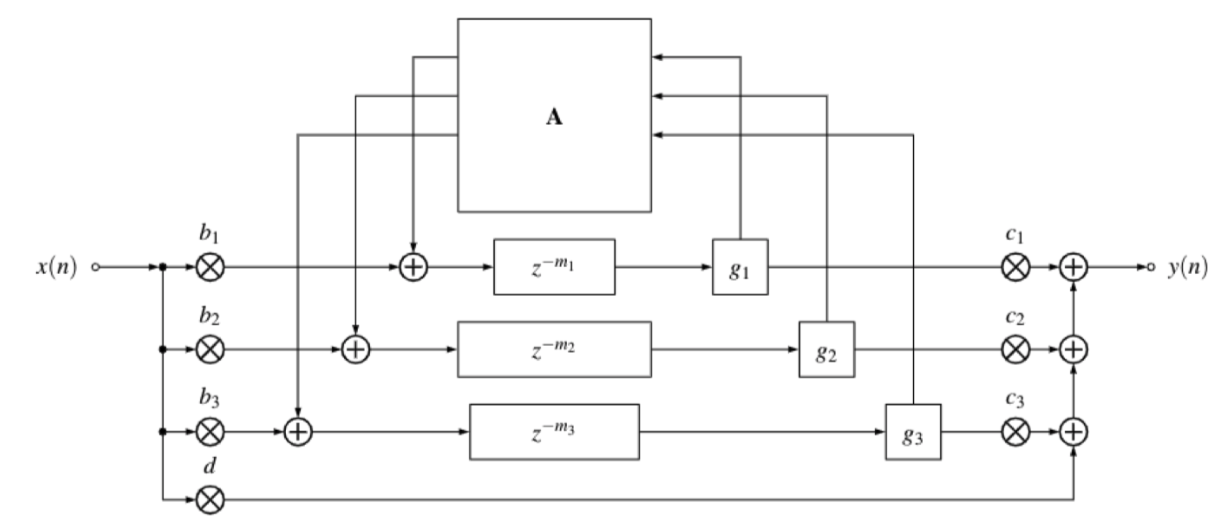
\includegraphics{images/fdn_diagram.png}
\caption{fdn\_diagram}
\end{figure}

The lossless recirculating matrix could be the Hadamard matrix for
example.

\[
H_{4}=\left[ \begin{array}{cccc}{1} & {1} & {1} & {1} \\ {1} & {-1} & {1} & {-1} \\ {1} & {1} & {-1} & {-1} \\ {1} & {-1} & {-1} & {1}\end{array}\right]
\]

    I wrote a Python version of FDN written by T.Lokki. This is incomplete
but I do not have the time to improve it.

    \begin{Verbatim}[commandchars=\\\{\}]
{\color{incolor}In [{\color{incolor}77}]:} \PY{c+c1}{\PYZsh{} Feedback Delay Network by T.Lokki}
         
         \PY{l+s+sd}{\PYZsq{}\PYZsq{}\PYZsq{}}
         \PY{l+s+sd}{Matlab version from DAFX pg.170}
         
         \PY{l+s+sd}{\PYZpc{} delaynetwork.m}
         \PY{l+s+sd}{\PYZpc{} Author: T. Lokki }
         \PY{l+s+sd}{fs=44100;}
         \PY{l+s+sd}{gain=0.97;}
         
         \PY{l+s+sd}{\PYZpc{} Create an impulse}
         \PY{l+s+sd}{x = zeros(1,1*fs); }
         \PY{l+s+sd}{x(1) = 1; }
         \PY{l+s+sd}{y = zeros(1,fs);}
         \PY{l+s+sd}{b = [1 1 1 1];}
         \PY{l+s+sd}{c = [0.8 0.8 0.8 0.8];}
         
         \PY{l+s+sd}{\PYZpc{} Feedback matrix}
         \PY{l+s+sd}{a(1,:)=[0 1 1 0]; }
         \PY{l+s+sd}{a(2,:)=[\PYZhy{}1 0 0 \PYZhy{}1]; }
         \PY{l+s+sd}{a(3,:)=[1 0 0 \PYZhy{}1]; }
         \PY{l+s+sd}{a(4,:)=[0 1 \PYZhy{}1 0]; }
         \PY{l+s+sd}{a2=a*(1/sqrt(2)) * gain;}
         
         \PY{l+s+sd}{\PYZpc{} Delay lines, use prime}
         
         \PY{l+s+sd}{m=[149 211 263 293]\PYZsq{}; }
         \PY{l+s+sd}{z1=zeros(1,max(max(m))); }
         \PY{l+s+sd}{z2=zeros(1,max(max(m))); }
         \PY{l+s+sd}{z3=zeros(1,max(max(m))); }
         \PY{l+s+sd}{z4=zeros(1,max(max(m)));}
         
         \PY{l+s+sd}{for n = 1:length(y)}
         \PY{l+s+sd}{    tmp = [z1(m(1)) z2(m(2)) z3(m(3)) z4(m(4))]; }
         \PY{l+s+sd}{    y(n) = x(n) + c(1)*z1(m(1)) + c(2)*z2(m(2)) + c(3)*z3(m(3)) + c(4)*z4(m(4));}
         \PY{l+s+sd}{    z1 = [(x(n)*b(1) + tmp*a2(1,:)\PYZsq{}) z1(1:length(z1)\PYZhy{}1)]; }
         \PY{l+s+sd}{    z2 = [(x(n)*b(2) + tmp*a2(2,:)\PYZsq{}) z2(1:length(z2)\PYZhy{}1)]; }
         \PY{l+s+sd}{    z3 = [(x(n)*b(3) + tmp*a2(3,:)\PYZsq{}) z3(1:length(z3)\PYZhy{}1)]; }
         \PY{l+s+sd}{    z4 = [(x(n)*b(4) + tmp*a2(4,:)\PYZsq{}) z4(1:length(z4)\PYZhy{}1)];}
         \PY{l+s+sd}{end }
         
         \PY{l+s+sd}{plot(y)}
         \PY{l+s+sd}{\PYZsq{}\PYZsq{}\PYZsq{}}
         
         \PY{n}{T60s} \PY{o}{=} \PY{p}{[}\PY{l+m+mf}{0.7}\PY{p}{,} \PY{l+m+mf}{0.14}\PY{p}{,} \PY{l+m+mf}{3.0}\PY{p}{,} \PY{l+m+mf}{0.6}\PY{p}{]}
         \PY{n}{fs} \PY{o}{=} \PY{l+m+mi}{44100}
         \PY{n}{gain} \PY{o}{=} \PY{l+m+mf}{0.97}
         \PY{n}{chunk} \PY{o}{=} \PY{l+m+mi}{4410}
         
         \PY{n}{violin} \PY{o}{=} \PY{n}{read\PYZus{}wave}\PY{p}{(}\PY{n}{config}\PY{o}{.}\PY{n}{paths}\PY{o}{.}\PY{n}{data}\PY{p}{[}\PY{l+m+mi}{2}\PY{p}{]}\PY{p}{)}
         \PY{n}{x} \PY{o}{=} \PY{n}{violin}\PY{o}{.}\PY{n}{ys}\PY{o}{.}\PY{n}{copy}\PY{p}{(}\PY{p}{)}
         \PY{n}{y} \PY{o}{=} \PY{n}{np}\PY{o}{.}\PY{n}{zeros\PYZus{}like}\PY{p}{(}\PY{n}{x}\PY{p}{)}
         \PY{n}{b} \PY{o}{=} \PY{n}{np}\PY{o}{.}\PY{n}{ones}\PY{p}{(}\PY{l+m+mi}{4}\PY{p}{)}
         \PY{n}{c} \PY{o}{=} \PY{n}{np}\PY{o}{.}\PY{n}{ones}\PY{p}{(}\PY{l+m+mi}{4}\PY{p}{)} \PY{o}{*} \PY{l+m+mf}{0.8}
         
         \PY{n}{A} \PY{o}{=} \PY{n}{np}\PY{o}{.}\PY{n}{array}\PY{p}{(}\PY{p}{[}
             \PY{p}{[}\PY{l+m+mi}{0}\PY{p}{,}\PY{l+m+mi}{1}\PY{p}{,}\PY{l+m+mi}{1}\PY{p}{,}\PY{l+m+mi}{0}\PY{p}{]}\PY{p}{,}
             \PY{p}{[}\PY{o}{\PYZhy{}}\PY{l+m+mi}{1}\PY{p}{,}\PY{l+m+mi}{0}\PY{p}{,}\PY{l+m+mi}{0}\PY{p}{,}\PY{o}{\PYZhy{}}\PY{l+m+mi}{1}\PY{p}{]}\PY{p}{,}
             \PY{p}{[}\PY{l+m+mi}{1}\PY{p}{,}\PY{l+m+mi}{0}\PY{p}{,}\PY{l+m+mi}{0}\PY{p}{,}\PY{o}{\PYZhy{}}\PY{l+m+mi}{1}\PY{p}{]}\PY{p}{,}
             \PY{p}{[}\PY{l+m+mi}{0}\PY{p}{,}\PY{l+m+mi}{1}\PY{p}{,}\PY{o}{\PYZhy{}}\PY{l+m+mi}{1}\PY{p}{,}\PY{l+m+mi}{0}\PY{p}{]}
         \PY{p}{]}\PY{p}{)}
         \PY{n}{A} \PY{o}{=} \PY{n}{A} \PY{o}{/} \PY{n}{np}\PY{o}{.}\PY{n}{sqrt}\PY{p}{(}\PY{l+m+mi}{2}\PY{p}{)} \PY{o}{*} \PY{n}{gain}
         
         \PY{n}{m} \PY{o}{=} \PY{n}{np}\PY{o}{.}\PY{n}{array}\PY{p}{(}\PY{p}{[}\PY{l+m+mi}{149}\PY{p}{,} \PY{l+m+mi}{211}\PY{p}{,} \PY{l+m+mi}{263}\PY{p}{,} \PY{l+m+mi}{293}\PY{p}{]}\PY{p}{)}\PY{o}{.}\PY{n}{T}\PY{p}{;}
         \PY{n}{z} \PY{o}{=} \PY{n}{np}\PY{o}{.}\PY{n}{zeros}\PY{p}{(}\PY{p}{(}\PY{l+m+mi}{4}\PY{p}{,} \PY{n}{np}\PY{o}{.}\PY{n}{max}\PY{p}{(}\PY{n}{m}\PY{p}{)}\PY{p}{)}\PY{p}{)}\PY{p}{;}
         
         \PY{k}{for} \PY{n}{n} \PY{o+ow}{in} \PY{n+nb}{range}\PY{p}{(}\PY{n}{y}\PY{o}{.}\PY{n}{size}\PY{p}{)}\PY{p}{:}
             \PY{n}{tmp} \PY{o}{=} \PY{n}{np}\PY{o}{.}\PY{n}{array}\PY{p}{(}\PY{p}{[}
                 \PY{n}{z}\PY{p}{[}\PY{l+m+mi}{0}\PY{p}{,}\PY{n}{m}\PY{p}{[}\PY{l+m+mi}{0}\PY{p}{]}\PY{o}{\PYZhy{}}\PY{l+m+mi}{1}\PY{p}{]}\PY{p}{,} 
                 \PY{n}{z}\PY{p}{[}\PY{l+m+mi}{1}\PY{p}{,}\PY{n}{m}\PY{p}{[}\PY{l+m+mi}{1}\PY{p}{]}\PY{o}{\PYZhy{}}\PY{l+m+mi}{1}\PY{p}{]}\PY{p}{,} 
                 \PY{n}{z}\PY{p}{[}\PY{l+m+mi}{2}\PY{p}{,}\PY{n}{m}\PY{p}{[}\PY{l+m+mi}{2}\PY{p}{]}\PY{o}{\PYZhy{}}\PY{l+m+mi}{1}\PY{p}{]}\PY{p}{,} 
                 \PY{n}{z}\PY{p}{[}\PY{l+m+mi}{3}\PY{p}{,}\PY{n}{m}\PY{p}{[}\PY{l+m+mi}{3}\PY{p}{]}\PY{o}{\PYZhy{}}\PY{l+m+mi}{1}\PY{p}{]}\PY{p}{,} 
             \PY{p}{]}\PY{p}{)}
             
             \PY{n}{y}\PY{p}{[}\PY{n}{n}\PY{p}{]} \PY{o}{=} \PY{n}{x}\PY{p}{[}\PY{n}{n}\PY{p}{]} \PY{o}{+} \PY{n}{c}\PY{p}{[}\PY{l+m+mi}{0}\PY{p}{]} \PY{o}{*} \PY{n}{z}\PY{p}{[}\PY{l+m+mi}{0}\PY{p}{]}\PY{p}{[}\PY{n}{m}\PY{p}{[}\PY{l+m+mi}{0}\PY{p}{]}\PY{o}{\PYZhy{}}\PY{l+m+mi}{1}\PY{p}{]} \PYZbs{}
                         \PY{o}{+} \PY{n}{c}\PY{p}{[}\PY{l+m+mi}{1}\PY{p}{]} \PY{o}{*} \PY{n}{z}\PY{p}{[}\PY{l+m+mi}{1}\PY{p}{]}\PY{p}{[}\PY{n}{m}\PY{p}{[}\PY{l+m+mi}{1}\PY{p}{]}\PY{o}{\PYZhy{}}\PY{l+m+mi}{1}\PY{p}{]} \PYZbs{}
                         \PY{o}{+} \PY{n}{c}\PY{p}{[}\PY{l+m+mi}{2}\PY{p}{]} \PY{o}{*} \PY{n}{z}\PY{p}{[}\PY{l+m+mi}{2}\PY{p}{]}\PY{p}{[}\PY{n}{m}\PY{p}{[}\PY{l+m+mi}{2}\PY{p}{]}\PY{o}{\PYZhy{}}\PY{l+m+mi}{1}\PY{p}{]} \PYZbs{}
                         \PY{o}{+} \PY{n}{c}\PY{p}{[}\PY{l+m+mi}{3}\PY{p}{]} \PY{o}{*} \PY{n}{z}\PY{p}{[}\PY{l+m+mi}{3}\PY{p}{]}\PY{p}{[}\PY{n}{m}\PY{p}{[}\PY{l+m+mi}{3}\PY{p}{]}\PY{o}{\PYZhy{}}\PY{l+m+mi}{1}\PY{p}{]} 
             \PY{n}{z}\PY{p}{[}\PY{p}{:}\PY{p}{,}\PY{l+m+mi}{1}\PY{p}{:}\PY{p}{]} \PY{o}{=} \PY{n}{z}\PY{p}{[}\PY{p}{:}\PY{p}{,}\PY{p}{:}\PY{n}{np}\PY{o}{.}\PY{n}{max}\PY{p}{(}\PY{n}{m}\PY{p}{)}\PY{o}{\PYZhy{}}\PY{l+m+mi}{1}\PY{p}{]}
             \PY{n}{z}\PY{p}{[}\PY{p}{:}\PY{p}{,}\PY{l+m+mi}{0}\PY{p}{]} \PY{o}{=} \PY{n}{x}\PY{p}{[}\PY{n}{n}\PY{p}{]} \PY{o}{*} \PY{n}{b} \PY{o}{+} \PY{p}{(}\PY{n}{tmp} \PY{o}{@} \PY{n}{A}\PY{p}{)}
         \PY{c+c1}{\PYZsh{}     z[0,0] = x[n] * b[0] + (tmp @ A[0])}
         \PY{c+c1}{\PYZsh{}     z[1,0] = x[n] * b[1] + (tmp @ A[1])}
         \PY{c+c1}{\PYZsh{}     z[2,0] = x[n] * b[2] + (tmp @ A[2])}
         \PY{c+c1}{\PYZsh{}     z[3,0] = x[n] * b[3] + (tmp @ A[3])}
             
         \PY{n}{plt}\PY{o}{.}\PY{n}{plot}\PY{p}{(}\PY{n}{y}\PY{p}{)}
         \PY{n}{violin}\PY{o}{.}\PY{n}{ys} \PY{o}{=} \PY{n}{y}
         \PY{n}{violin}\PY{o}{.}\PY{n}{make\PYZus{}audio}\PY{p}{(}\PY{p}{)}
\end{Verbatim}


\begin{Verbatim}[commandchars=\\\{\}]
{\color{outcolor}Out[{\color{outcolor}77}]:} <IPython.lib.display.Audio object>
\end{Verbatim}
            
    \begin{center}
    \adjustimage{max size={0.9\linewidth}{0.9\paperheight}}{output_14_1.png}
    \end{center}
    { \hspace*{\fill} \\}
    
    \begin{Verbatim}[commandchars=\\\{\}]
{\color{incolor}In [{\color{incolor}78}]:} \PY{k+kn}{from} \PY{n+nn}{scipy}\PY{n+nn}{.}\PY{n+nn}{io} \PY{k}{import} \PY{n}{wavfile}
\end{Verbatim}


    \begin{Verbatim}[commandchars=\\\{\}]
{\color{incolor}In [{\color{incolor}79}]:} \PY{n}{wavfile}\PY{o}{.}\PY{n}{write}\PY{p}{(}\PY{l+s+s2}{\PYZdq{}}\PY{l+s+s2}{violin\PYZus{}fdn.wav}\PY{l+s+s2}{\PYZdq{}}\PY{p}{,} \PY{l+m+mi}{44100}\PY{p}{,} \PY{n}{y}\PY{p}{)}
\end{Verbatim}


    \begin{Verbatim}[commandchars=\\\{\}]
{\color{incolor}In [{\color{incolor}74}]:} \PY{n}{plt}\PY{o}{.}\PY{n}{plot}\PY{p}{(}\PY{n}{y\PYZus{}reference}\PY{p}{)}
\end{Verbatim}


\begin{Verbatim}[commandchars=\\\{\}]
{\color{outcolor}Out[{\color{outcolor}74}]:} [<matplotlib.lines.Line2D at 0x1c24195a90>]
\end{Verbatim}
            
    \begin{center}
    \adjustimage{max size={0.9\linewidth}{0.9\paperheight}}{output_17_1.png}
    \end{center}
    { \hspace*{\fill} \\}
    
    \hypertarget{references}{%
\subsection{References}\label{references}}

\begin{itemize}
\tightlist
\item
  DAFX: Digital Audio Effects by John Wiley
\end{itemize}


    % Add a bibliography block to the postdoc
    
    
    
    \end{document}
